\documentclass[12pt,preprint, authoryear]{elsarticle}

\usepackage{lmodern}
%%%% My spacing
\usepackage{setspace}
\setstretch{1.5}
\DeclareMathSizes{12}{14}{10}{10}

% Wrap around which gives all figures included the [H] command, or places it "here". This can be tedious to code in Rmarkdown.
\usepackage{float}
\let\origfigure\figure
\let\endorigfigure\endfigure
\renewenvironment{figure}[1][2] {
    \expandafter\origfigure\expandafter[H]
} {
    \endorigfigure
}

\let\origtable\table
\let\endorigtable\endtable
\renewenvironment{table}[1][2] {
    \expandafter\origtable\expandafter[H]
} {
    \endorigtable
}


\usepackage{ifxetex,ifluatex}
\usepackage{fixltx2e} % provides \textsubscript
\ifnum 0\ifxetex 1\fi\ifluatex 1\fi=0 % if pdftex
  \usepackage[T1]{fontenc}
  \usepackage[utf8]{inputenc}
\else % if luatex or xelatex
  \ifxetex
    \usepackage{mathspec}
    \usepackage{xltxtra,xunicode}
  \else
    \usepackage{fontspec}
  \fi
  \defaultfontfeatures{Mapping=tex-text,Scale=MatchLowercase}
  \newcommand{\euro}{€}
\fi

\usepackage{amssymb, amsmath, amsthm, amsfonts}

\def\bibsection{\section*{References}} %%% Make "References" appear before bibliography


\usepackage[round]{natbib}

\usepackage{longtable}
\usepackage[margin=2.3cm,bottom=2cm,top=2.5cm, includefoot]{geometry}
\usepackage{fancyhdr}
\usepackage[bottom, hang, flushmargin]{footmisc}
\usepackage{graphicx}
\numberwithin{equation}{section}
\numberwithin{figure}{section}
\numberwithin{table}{section}
\setlength{\parindent}{0cm}
\setlength{\parskip}{1.3ex plus 0.5ex minus 0.3ex}
\usepackage{textcomp}
\renewcommand{\headrulewidth}{0.2pt}
\renewcommand{\footrulewidth}{0.3pt}

\usepackage{array}
\newcolumntype{x}[1]{>{\centering\arraybackslash\hspace{0pt}}p{#1}}

%%%%  Remove the "preprint submitted to" part. Don't worry about this either, it just looks better without it:
\makeatletter
\def\ps@pprintTitle{%
  \let\@oddhead\@empty
  \let\@evenhead\@empty
  \let\@oddfoot\@empty
  \let\@evenfoot\@oddfoot
}
\makeatother

 \def\tightlist{} % This allows for subbullets!

\usepackage{hyperref}
\hypersetup{breaklinks=true,
            bookmarks=true,
            colorlinks=true,
            citecolor=blue,
            urlcolor=blue,
            linkcolor=blue,
            pdfborder={0 0 0}}


% The following packages allow huxtable to work:
\usepackage{siunitx}
\usepackage{multirow}
\usepackage{hhline}
\usepackage{calc}
\usepackage{tabularx}
\usepackage{booktabs}
\usepackage{caption}


\newenvironment{columns}[1][]{}{}

\newenvironment{column}[1]{\begin{minipage}{#1}\ignorespaces}{%
\end{minipage}
\ifhmode\unskip\fi
\aftergroup\useignorespacesandallpars}

\def\useignorespacesandallpars#1\ignorespaces\fi{%
#1\fi\ignorespacesandallpars}

\makeatletter
\def\ignorespacesandallpars{%
  \@ifnextchar\par
    {\expandafter\ignorespacesandallpars\@gobble}%
    {}%
}
\makeatother

\newlength{\cslhangindent}
\setlength{\cslhangindent}{1.5em}
\newenvironment{CSLReferences}%
  {\setlength{\parindent}{0pt}%
  \everypar{\setlength{\hangindent}{\cslhangindent}}\ignorespaces}%
  {\par}


\urlstyle{same}  % don't use monospace font for urls
\setlength{\parindent}{0pt}
\setlength{\parskip}{6pt plus 2pt minus 1pt}
\setlength{\emergencystretch}{3em}  % prevent overfull lines
\setcounter{secnumdepth}{5}

%%% Use protect on footnotes to avoid problems with footnotes in titles
\let\rmarkdownfootnote\footnote%
\def\footnote{\protect\rmarkdownfootnote}
\IfFileExists{upquote.sty}{\usepackage{upquote}}{}

%%% Include extra packages specified by user

%%% Hard setting column skips for reports - this ensures greater consistency and control over the length settings in the document.
%% page layout
%% paragraphs
\setlength{\baselineskip}{12pt plus 0pt minus 0pt}
\setlength{\parskip}{12pt plus 0pt minus 0pt}
\setlength{\parindent}{0pt plus 0pt minus 0pt}
%% floats
\setlength{\floatsep}{12pt plus 0 pt minus 0pt}
\setlength{\textfloatsep}{20pt plus 0pt minus 0pt}
\setlength{\intextsep}{14pt plus 0pt minus 0pt}
\setlength{\dbltextfloatsep}{20pt plus 0pt minus 0pt}
\setlength{\dblfloatsep}{14pt plus 0pt minus 0pt}
%% maths
\setlength{\abovedisplayskip}{12pt plus 0pt minus 0pt}
\setlength{\belowdisplayskip}{12pt plus 0pt minus 0pt}
%% lists
\setlength{\topsep}{10pt plus 0pt minus 0pt}
\setlength{\partopsep}{3pt plus 0pt minus 0pt}
\setlength{\itemsep}{5pt plus 0pt minus 0pt}
\setlength{\labelsep}{8mm plus 0mm minus 0mm}
\setlength{\parsep}{\the\parskip}
\setlength{\listparindent}{\the\parindent}
%% verbatim
\setlength{\fboxsep}{5pt plus 0pt minus 0pt}



\begin{document}



\begin{frontmatter}  %

\title{Question 1}

% Set to FALSE if wanting to remove title (for submission)




\author[Add1]{Sahil Bhugwan}
\ead{}





\address[Add1]{Github-\url{https://github.com/SBhugwan}}

\cortext[cor]{Corresponding author: Sahil Bhugwan}

\begin{abstract}
\small{
The Covid-19 pandemic has wreaked havoc on many facets of our lives, and
continue to affect travel, work and how people socially interact
}
\end{abstract}

\vspace{1cm}


\begin{keyword}
\footnotesize{
COVID-19 \\
\vspace{0.3cm}
}
\end{keyword}



\vspace{0.5cm}

\end{frontmatter}



%________________________
% Header and Footers
%%%%%%%%%%%%%%%%%%%%%%%%%%%%%%%%%
\pagestyle{fancy}
\chead{}
\rhead{}
\lfoot{}
\rfoot{\footnotesize Page \thepage}
\lhead{}
%\rfoot{\footnotesize Page \thepage } % "e.g. Page 2"
\cfoot{}

%\setlength\headheight{30pt}
%%%%%%%%%%%%%%%%%%%%%%%%%%%%%%%%%
%________________________

\headsep 35pt % So that header does not go over title




\hypertarget{introduction}{%
\section{\texorpdfstring{Introduction
\label{Introduction}}{Introduction }}\label{introduction}}

COVID-19 was a unique time in the wold with basically the whole world
going into a lock down. It therefore is crucial to look at how certain
countries performed we we take a particular look at how Africa did
compared to the rest of the world.

\hypertarget{africa}{%
\section{Africa}\label{africa}}

This section will look at how Africa does compared to the rest of the
world. It is important to note that in Africa they are more used to
responding to outbreaks fro example the Ebola outbreak.

First i will be looking at the average deaths compared to other regions

\begin{Shaded}
\begin{Highlighting}[]
\NormalTok{AVD}
\end{Highlighting}
\end{Shaded}

\begin{figure}

{\centering \includegraphics{Q1_files/figure-latex/Figure1-1} 

}

\caption{Average deaths \label{Figure1}}\label{fig:Figure1}
\end{figure}

It is clear that the average deaths in Africa seem to be much lower than
that to the rest of the world this suggesting that Africa might have
been quicker to respond to the infection rates. However it is important
to note that more people live outside of Africa. Though we could look at
other important consideration, just as testing of COVID.

\begin{Shaded}
\begin{Highlighting}[]
\NormalTok{TP}
\end{Highlighting}
\end{Shaded}

\begin{figure}

{\centering \includegraphics{Q1_files/figure-latex/Figure2-1} 

}

\caption{Testing rates \label{Figure2}}\label{fig:Figure2}
\end{figure}

This graph shows that Africa had less test on average compared to the
rest of the world. This could mean that on average Africa could have had
less positive case of Covid compared to the world. Which wold make
intuitive sense given the fact that Africa does have less people that of
the rest of the world.

\hypertarget{healthcare-capacity-in-africa}{%
\subsection{Healthcare capacity in
Africa}\label{healthcare-capacity-in-africa}}

In these section we will look in term ``hospitals'' in how Africa
performed compared to the rest of the World. The first thing that i will
look at is how many hospital beds

\begin{Shaded}
\begin{Highlighting}[]
\NormalTok{HB}
\end{Highlighting}
\end{Shaded}

\begin{figure}

{\centering 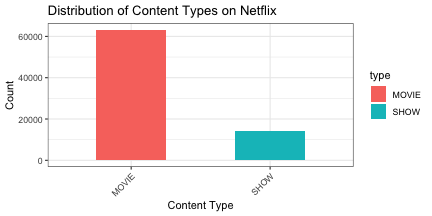
\includegraphics{Q1_files/figure-latex/Figure3-1} 

}

\caption{Hospital Beds \label{Figure3}}\label{fig:Figure3}
\end{figure}

It is clear that when COVID hit the world the number of bed needed
increased dramatically however the increase was more prominent in other
regions outside of Africa. The could be due to numerous reasons. A
possibility could be the fact that in Africa they had less ICU patients
compared to the rest of the World.

\begin{Shaded}
\begin{Highlighting}[]
\NormalTok{HCC}
\end{Highlighting}
\end{Shaded}

\begin{figure}

{\centering \includegraphics{Q1_files/figure-latex/Figure4-1} 

}

\caption{ICU Patients \label{Figure4}}\label{fig:Figure4}
\end{figure}

It is clear that Africa didn't have such a large spike in ICU patients
than the rest of the world. What we can gather from this is that Africa
was handled the pandemic efficiently in that it was quick to respond to
the first outbreak and was able to control the spread of it.

\begin{Shaded}
\begin{Highlighting}[]
\NormalTok{HFvICU}
\end{Highlighting}
\end{Shaded}

\begin{figure}

{\centering \includegraphics{Q1_files/figure-latex/Figure5-1} 

}

\caption{Hospitalization VS ICU Admissions  \label{Figure5}}\label{fig:Figure5}
\end{figure}

\begin{Shaded}
\begin{Highlighting}[]
\NormalTok{SHFICU}
\end{Highlighting}
\end{Shaded}

\begin{figure}

{\centering \includegraphics{Q1_files/figure-latex/Figure6-1} 

}

\caption{Hospitalization VS ICU Admissions  \label{Figure6}}\label{fig:Figure6}
\end{figure}

There by looking at the two graph that Africa responded much quicker
that that of the rest of the world to increase its hospital facilities
to cope with the increase in ICU patients.

This shows that AFrica on probabary also didnt have as many people
infected or that when there was a vaccine the number of new cases to
people was under control.

\begin{Shaded}
\begin{Highlighting}[]
\NormalTok{MCFV}
\end{Highlighting}
\end{Shaded}

\begin{figure}

{\centering \includegraphics{Q1_files/figure-latex/Figure7-1} 

}

\caption{ Ave cases vs vaccinated  \label{Figure7}}\label{fig:Figure7}
\end{figure}

Therefore we can see that in Africa the proportion on new case to people
vaccinated remained relatively closed togethor and didnt get out of
control.

An intersting observation will be to look at the impact of the
intervention.

\begin{Shaded}
\begin{Highlighting}[]
\NormalTok{SI}
\end{Highlighting}
\end{Shaded}

\begin{figure}

{\centering \includegraphics{Q1_files/figure-latex/Figure8-1} 

}

\caption{ Ave cases vs vaccinated  \label{Figure8 }}\label{fig:Figure8}
\end{figure}

The stringency index is a composite measurebased on nine response
indicators including schoolclosures, workplace closures, and travel
bans. This shows how effective the interventions where with regards to
controlloing the pandemic.

\hypertarget{poverty-levels}{%
\section{Poverty levels}\label{poverty-levels}}

Next i will be looking to see if specific groups for example those in
extreme poverty had it worse

\begin{Shaded}
\begin{Highlighting}[]
\NormalTok{EPL}
\end{Highlighting}
\end{Shaded}

\begin{figure}

{\centering \includegraphics{Q1_files/figure-latex/Figure9-1} 

}

\caption{ Extreme poverty  \label{Figure9 }}\label{fig:Figure9}
\end{figure}

Next i will look at Perform analysis based on life expectancy

\begin{Shaded}
\begin{Highlighting}[]
\NormalTok{LE}
\end{Highlighting}
\end{Shaded}

\begin{figure}

{\centering \includegraphics{Q1_files/figure-latex/Figure10-1} 

}

\caption{Life Expectancy \label{Figure10}}\label{fig:Figure10}
\end{figure}

\hypertarget{conclusion}{%
\section{Conclusion}\label{conclusion}}

\bibliography{Tex/ref}





\end{document}
